\documentclass[12pt]{exam}

\usepackage[margin=1in]{geometry}

\newcommand{\class}{PHYS 202}
\newcommand{\term}{Fall 2021}
\newcommand{\examnum}{CO4c (v2)}
\newcommand{\examdate}{\today}
\newcommand{\timelimit}{60 Minutes}


% Engine-specific settings
% Detect pdftex/xetex/luatex, and load appropriate font packages.
% This is inspired by the approach in the iftex package.
% pdftex:
\ifx\pdfmatch\undefined
\else
    \usepackage[T1]{fontenc}
    \usepackage[utf8]{inputenc}
\fi
% xetex:
\ifx\XeTeXinterchartoks\undefined
\else
    \usepackage{fontspec}
    \defaultfontfeatures{Ligatures=TeX}
\fi
% luatex:
\ifx\directlua\undefined
\else
    \usepackage{fontspec}
\fi
% End engine-specific settings

\usepackage{amsmath,amssymb}
\usepackage{fullpage}
\usepackage{graphicx}
\usepackage[svgnames]{xcolor}
\usepackage{url}
\urlstyle{same}

\usepackage{pythontex}
% \restartpythontexsession{\thesection}


\usepackage[framemethod=TikZ]{mdframed}

\newcommand{\pytex}{Python\TeX}
\renewcommand*{\thefootnote}{\fnsymbol{footnote}}

%\usepackage{circuitikz}
\usepackage{siunitx}
\usepackage{pgfplots}
\usepackage{nopageno}



\begin{document}

%\noindent
%\begin{tabular}{l r}
%\textbf{\class} - \textbf{\examnum}  & \textbf{Name} \makebox[3.25in]{\hrulefill}  \\
%\textbf{\term} &&\\
%\textbf{\examnum} &&\\
%\textbf{\examdate} &&\\
%\textbf{Time Limit: \timelimit} & Teaching Assistant & \makebox[2in]{\hrulefill}
%\end{tabular}\\
%\rule[1ex]{\textwidth}{2.21pt}

%\pagestyle{head}
%\firstpageheader{}{}{}
%\runningheader{\class}{\examnum\ }{Page \thepage\ of \numpages}
%\runningheadrule


%\begin{questions}
%\question 

\begin{pycode}
from pylab import *
import random

from randassign import RandAssign
ra = RandAssign()

def make_problem():
	# Random values for this problem
	def rand_mass():
		return round(uniform(1,3),2)
	def rand_length():
		return round(uniform(.05,.39),2)
	def rand_accel():
		return round(uniform(4,8),2)
	def rand_spring():
		return random.randrange(10,65)	

		
	mass = rand_mass()
	length = rand_length()
	accel = rand_accel()
	spring = rand_spring()


		
	problem_template = r'''
	An object attached to an ideal massless spring is pulled across a frictionless surface. If the mass of the object is $m = \SI{{{0:.3g}}}{{\kilogram}} $ and the spring is stretched by $\SI{{{1:.3g}}}{{\meter}}$ when the object is accelerating at $\SI{{{2:.3g}}}{{\meter/\second^2}}$, what is the spring constant?
	'''
	
	## SOLUTION CODE HAS BEEN WRITTEN below
	s = mass* accel / length 

	problem = problem_template.format(mass,length,accel,spring)
	
	return(problem,s)
#	return(problem)
	
## Generate 4 unique problems
## The chance of two identical problems is very low in this case
## But checking for identical problems won't hurt
problems = []
while len(problems) < 4:
    p,m = make_problem()
    if p not in problems:
        problems.append(p)
        t = '\\SI{{{0:.3g}}}{{\\kilogram}}'
        ra.addsoln(t.format(m))

#print('\\begin{questions}')
for n, p in enumerate(problems):
    print('\\noindent \\begin{tabular}{l l r} \\textbf{\\class} - \\textbf{\\examnum}  & \\textbf{Name} \\makebox[3.25in]{\\hrulefill}  \\\\ \\end{tabular} \\\\ \\rule[1ex]{\\textwidth}{2.21pt} \\begin{questions}\\question '+ p + '\\end{questions}\\newpage')
    if n+1 < len(problems):
        print(r'\vspace{1in}')
#print('\\end{questions}')

#p = make_problem()
#t = '\\SI{{{0:.3g}}}{{\\volt}} and \\SI{{{1:.3g}}}{{\\volt}}and \\SI{{{2:.3g}}}{{\\volt}} and \\SI{{{3:.3g}}}{{\\volt}} and \\SI{{{4:.3g}}}{{\\ampere}} and \\SI{{{5:.3g}}}{{\\ampere}} and \\SI{{{6:.3g}}}{{\\ampere}} and \\SI{{{7:.3g}}}{{\\ampere}}, and \\SI{{{8:.3g}}}{{\\watt}}, and \\SI{{{9:.3g}}}{{\\watt}}, and \\SI{{{10:.3g}}}{{\\watt}} and \\SI{{{11:.3g}}}{{\\watt}}'
#ra.addsoln(t.format(v1,v2,v3,v4,i1,i2,i3,i4,w1,w2,w3,w4))

#print('\\begin{questions}\\question '+ p + '\\end{questions}')

\end{pycode}

\newpage


\begin{pycode}
from pylab import *
import random

from randassign import RandAssign
ra = RandAssign()

def make_problem():
	# Random values for this problem
	def rand_mass():
		return round(uniform(1,3),2)
	def rand_length():
		return round(uniform(.05,.39),2)
	def rand_accel():
		return round(uniform(4,8),2)
	def rand_spring():
		return random.randrange(10,65)	

		
	mass = rand_mass()
	length = rand_length()
	accel = rand_accel()
	spring = rand_spring()


		
	problem_template = r'''
	An object attached to an ideal massless spring is pulled across a frictionless surface. If the spring constant is $k = \SI{{{3:.3g}}}{{\newton/\meter}} $ and the spring is stretched by $\SI{{{1:.3g}}}{{\meter}}$ when the object is accelerating at $\SI{{{2:.3g}}}{{\meter/\second^2}}$, what is the mass of the object?
	'''
	
	## SOLUTION CODE HAS BEEN WRITTEN below
	m = spring * length / accel

	problem = problem_template.format(mass,length,accel,spring)
	
	return(problem,m)
#	return(problem)
	
## Generate 4 unique problems
## The chance of two identical problems is very low in this case
## But checking for identical problems won't hurt
problems = []
while len(problems) < 4:
    p,m = make_problem()
    if p not in problems:
        problems.append(p)
        t = '\\SI{{{0:.3g}}}{{\\kilogram}}'
        ra.addsoln(t.format(m))

#print('\\begin{questions}')
for n, p in enumerate(problems):
    print('\\noindent \\begin{tabular}{l l r} \\textbf{\\class} - \\textbf{\\examnum}  & \\textbf{Name} \\makebox[3.25in]{\\hrulefill}  \\\\ \\end{tabular} \\\\ \\rule[1ex]{\\textwidth}{2.21pt} \\begin{questions}\\question '+ p + '\\end{questions}\\newpage')
    if n+1 < len(problems):
        print(r'\vspace{1in}')
#print('\\end{questions}')

#p = make_problem()
#t = '\\SI{{{0:.3g}}}{{\\volt}} and \\SI{{{1:.3g}}}{{\\volt}}and \\SI{{{2:.3g}}}{{\\volt}} and \\SI{{{3:.3g}}}{{\\volt}} and \\SI{{{4:.3g}}}{{\\ampere}} and \\SI{{{5:.3g}}}{{\\ampere}} and \\SI{{{6:.3g}}}{{\\ampere}} and \\SI{{{7:.3g}}}{{\\ampere}}, and \\SI{{{8:.3g}}}{{\\watt}}, and \\SI{{{9:.3g}}}{{\\watt}}, and \\SI{{{10:.3g}}}{{\\watt}} and \\SI{{{11:.3g}}}{{\\watt}}'
#ra.addsoln(t.format(v1,v2,v3,v4,i1,i2,i3,i4,w1,w2,w3,w4))

#print('\\begin{questions}\\question '+ p + '\\end{questions}')

\end{pycode}

\newpage


\begin{pycode}
from pylab import *
import random

from randassign import RandAssign
ra = RandAssign()

def make_problem():
	# Random values for this problem
	def rand_mass():
		return round(uniform(1,3),2)
	def rand_length():
		return round(uniform(.5,3),2)
	def rand_speed():
		return round(uniform(0.15,0.45),2)
	def rand_angle():
		return random.randrange(25,40)
	def rand_k():
		return random.randrange(19,51)	

		
	mass = rand_mass()
	length = rand_length()
	speed = rand_speed()
	angle = rand_angle()
	spring = rand_k()


		
	problem_template = r'''
	Two identical springs with spring constant $k = \SI{{{4:.3g}}}{{\newton/\meter}} $ hold a $\SI{{{0:.3g}}}{{\kilogram}}$ hanging mass as in the figure below. Suppose $\theta =\ang{{{3:.3g}}}$. How much has one of the springs been stretched from its original length?
	'''
	
	## NO SOLUTION CODE HAS BEEN WRITTEN (YET)

	problem = problem_template.format(mass,length,speed,angle,spring)
	
#	return(problem,V1,V2,V3,V4,I1,I2,I3,I4,W1,W2,W3,W4)
	return(problem)
	
## Generate 4 unique problems
## The chance of two identical problems is very low in this case
## But checking for identical problems won't hurt
problems = []
while len(problems) < 4:
    p = make_problem()
    if p not in problems:
        problems.append(p)
#        t = '\\SI{{{0:.3g}}}{{\\volt}} and \\SI{{{1:.3g}}}{{\\volt}}and \\SI{{{2:.3g}}}{{\\volt}} and \\SI{{{3:.3g}}}{{\\volt}} and \\SI{{{4:.3g}}}{{\\volt}} and \\SI{{{5:.3g}}}{{\\ampere}} and \\SI{{{6:.3g}}}{{\\ampere}} and \\SI{{{7:.3g}}}{{\\ampere}} and \\SI{{{8:.3g}}}{{\\ampere}} and \\SI{{{9:.3g}}}{{\\ampere}}'
#        ra.addsoln(t.format(v1,v2,v3,v4,v5,i1,i2,i3,i4,i5))

#print('\\begin{questions}')
for n, p in enumerate(problems):
    print('\\noindent \\begin{tabular}{l l r} \\textbf{\\class} - \\textbf{\\examnum}  & \\textbf{Name} \\makebox[3.25in]{\\hrulefill}  \\\\ \\end{tabular} \\\\ \\rule[1ex]{\\textwidth}{2.21pt} \\begin{questions}\\setcounter{question}{1}\\question '+ p + '\\begin{figure}[h]\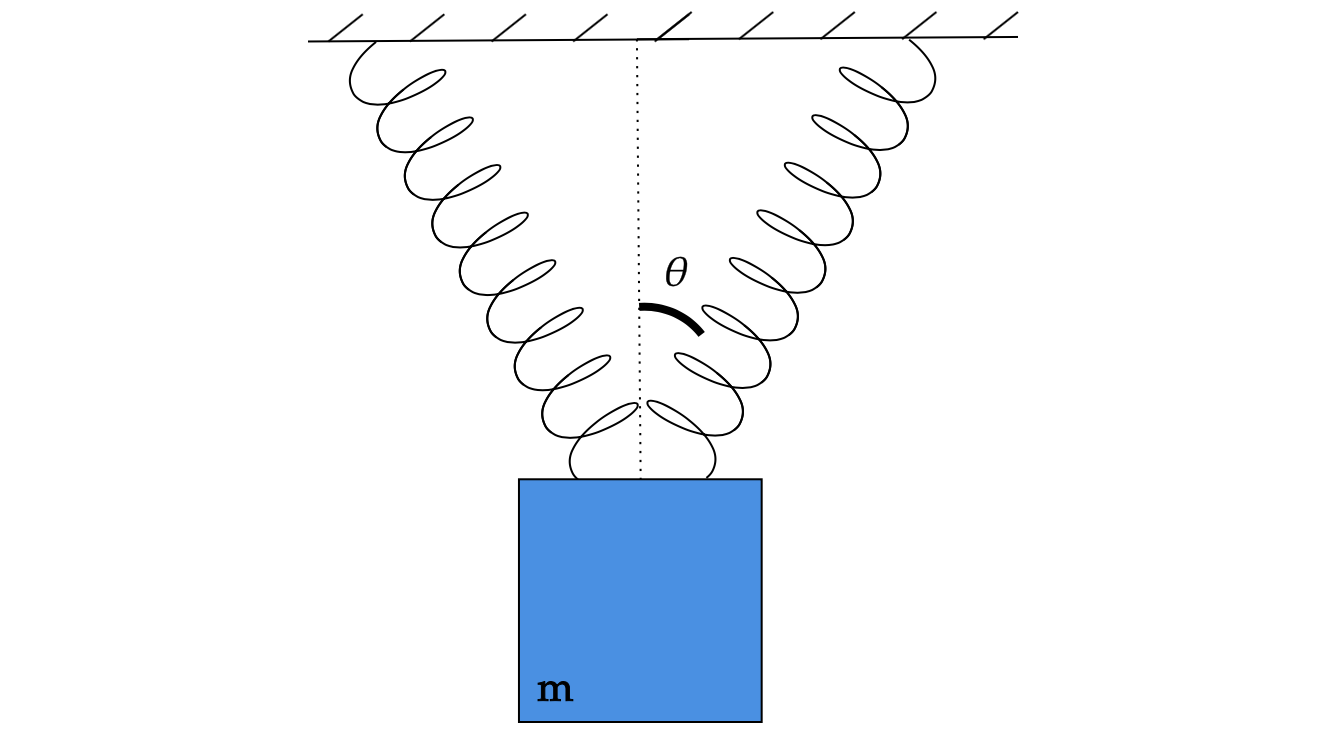
\includegraphics[width=10cm,keepaspectratio]{diagram-springs}\\end{figure}\\end{questions}\\newpage')
    if n+1 < len(problems):
        print(r'\vspace{1in}')
#print('\\end{questions}')

#p = make_problem()
#t = '\\SI{{{0:.3g}}}{{\\volt}} and \\SI{{{1:.3g}}}{{\\volt}}and \\SI{{{2:.3g}}}{{\\volt}} and \\SI{{{3:.3g}}}{{\\volt}} and \\SI{{{4:.3g}}}{{\\ampere}} and \\SI{{{5:.3g}}}{{\\ampere}} and \\SI{{{6:.3g}}}{{\\ampere}} and \\SI{{{7:.3g}}}{{\\ampere}}, and \\SI{{{8:.3g}}}{{\\watt}}, and \\SI{{{9:.3g}}}{{\\watt}}, and \\SI{{{10:.3g}}}{{\\watt}} and \\SI{{{11:.3g}}}{{\\watt}}'
#ra.addsoln(t.format(v1,v2,v3,v4,i1,i2,i3,i4,w1,w2,w3,w4))

#print('\\begin{questions}\\question '+ p + '\\end{questions}')

\end{pycode}


\begin{pycode}
from pylab import *
import random

from randassign import RandAssign
ra = RandAssign()

def make_problem():
	# Random values for this problem
	def rand_mass():
		return round(uniform(1,3),2)
	def rand_length():
		return round(uniform(.02,.39),2)
	def rand_speed():
		return round(uniform(0.15,0.45),2)
	def rand_angle():
		return random.randrange(25,40)
	def rand_k():
		return random.randrange(19,51)	

		
	mass = rand_mass()
	length = rand_length()
	speed = rand_speed()
	angle = rand_angle()
	spring = rand_k()


		
	problem_template = r'''
	Two identical springs with spring constant $k = \SI{{{4:.3g}}}{{\newton/\meter}} $ hold a hanging object as in the figure below. Suppose $\theta =\ang{{{3:.3g}}}$ and that the springs have each been stretched $\SI{{{1:.3g}}}{{\meter}}$ from their original length. What is the mass of the object?
	'''
	
	## NO SOLUTION CODE HAS BEEN WRITTEN (YET)

	problem = problem_template.format(mass,length,speed,angle,spring)
	
#	return(problem,V1,V2,V3,V4,I1,I2,I3,I4,W1,W2,W3,W4)
	return(problem)
	
## Generate 4 unique problems
## The chance of two identical problems is very low in this case
## But checking for identical problems won't hurt
problems = []
while len(problems) < 4:
    p = make_problem()
    if p not in problems:
        problems.append(p)
#        t = '\\SI{{{0:.3g}}}{{\\volt}} and \\SI{{{1:.3g}}}{{\\volt}}and \\SI{{{2:.3g}}}{{\\volt}} and \\SI{{{3:.3g}}}{{\\volt}} and \\SI{{{4:.3g}}}{{\\volt}} and \\SI{{{5:.3g}}}{{\\ampere}} and \\SI{{{6:.3g}}}{{\\ampere}} and \\SI{{{7:.3g}}}{{\\ampere}} and \\SI{{{8:.3g}}}{{\\ampere}} and \\SI{{{9:.3g}}}{{\\ampere}}'
#        ra.addsoln(t.format(v1,v2,v3,v4,v5,i1,i2,i3,i4,i5))

#print('\\begin{questions}')
for n, p in enumerate(problems):
    print('\\noindent \\begin{tabular}{l l r} \\textbf{\\class} - \\textbf{\\examnum}  & \\textbf{Name} \\makebox[3.25in]{\\hrulefill}  \\\\ \\end{tabular} \\\\ \\rule[1ex]{\\textwidth}{2.21pt} \\begin{questions}\\setcounter{question}{1}\\question '+ p + '\\begin{figure}[h]\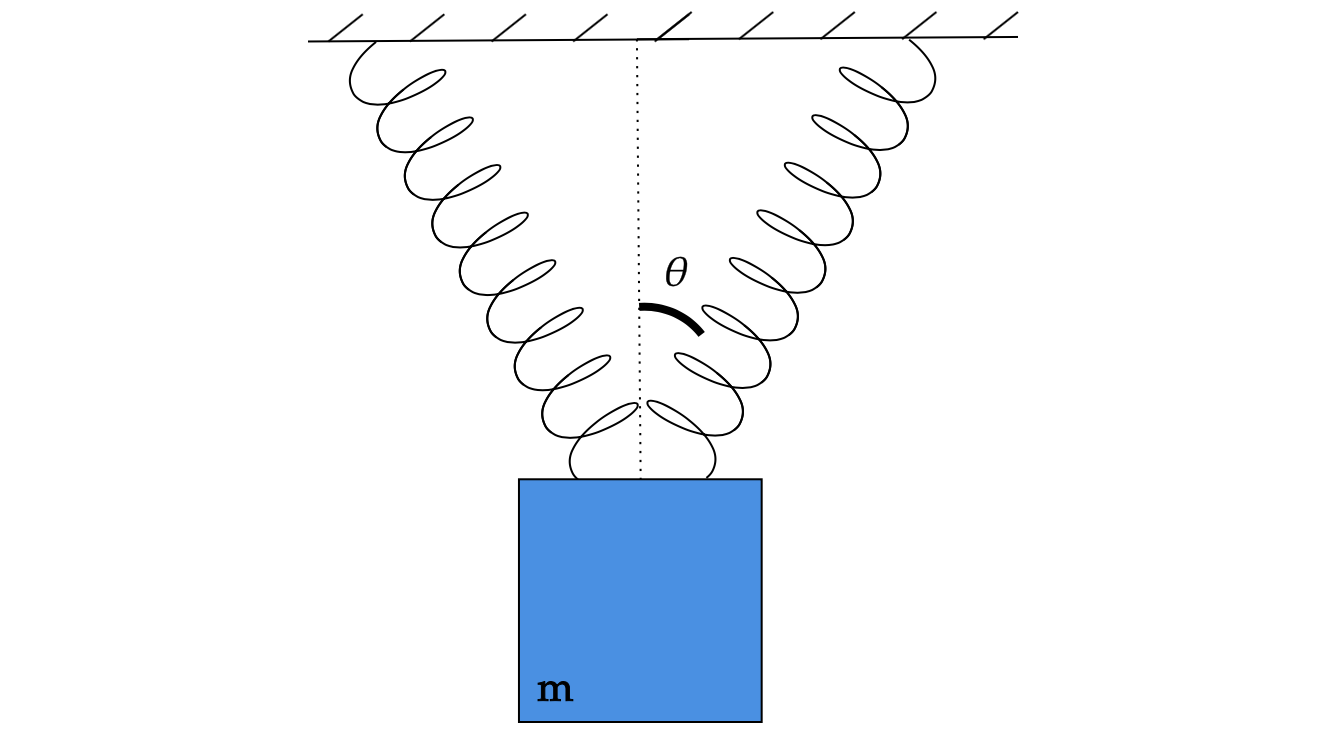
\includegraphics[width=10cm,keepaspectratio]{diagram-springs}\\end{figure}\\end{questions}\\newpage')
    if n+1 < len(problems):
        print(r'\vspace{1in}')
#print('\\end{questions}')

#p = make_problem()
#t = '\\SI{{{0:.3g}}}{{\\volt}} and \\SI{{{1:.3g}}}{{\\volt}}and \\SI{{{2:.3g}}}{{\\volt}} and \\SI{{{3:.3g}}}{{\\volt}} and \\SI{{{4:.3g}}}{{\\ampere}} and \\SI{{{5:.3g}}}{{\\ampere}} and \\SI{{{6:.3g}}}{{\\ampere}} and \\SI{{{7:.3g}}}{{\\ampere}}, and \\SI{{{8:.3g}}}{{\\watt}}, and \\SI{{{9:.3g}}}{{\\watt}}, and \\SI{{{10:.3g}}}{{\\watt}} and \\SI{{{11:.3g}}}{{\\watt}}'
#ra.addsoln(t.format(v1,v2,v3,v4,i1,i2,i3,i4,w1,w2,w3,w4))

#print('\\begin{questions}\\question '+ p + '\\end{questions}')

\end{pycode}

%\end{questions}
	
\end{document}
